\documentclass{article}

% if you need to pass options to natbib, use, e.g.:
\PassOptionsToPackage{numbers, compress}{natbib}
% before loading nips_2017
%
% to avoid loading the natbib package, add option nonatbib:
% \usepackage[nonatbib]{nips_2017}

\usepackage{nips_2018}

% to compile a camera-ready version, add the [final] option, e.g.:
% \usepackage[final]{nips_2017}

\usepackage[utf8]{inputenc} % allow utf-8 input
\usepackage[T1]{fontenc}    % use 8-bit T1 fonts
\usepackage{hyperref}       % hyperlinks
\usepackage{url}            % simple URL typesetting
\usepackage{booktabs}       % professional-quality tables
\usepackage{amsfonts}       % blackboard math symbols
\usepackage{nicefrac}       % compact symbols for 1/2, etc.
\usepackage{microtype}      % microtypography

\usepackage{hyperref}

\usepackage{amssymb}
\usepackage{amsmath}

% For citations
\usepackage{natbib}

% For figures
\usepackage{graphicx} % more modern
\usepackage{wrapfig}
%\usepackage{epsfig} % less modern
%\usepackage{subfigure} 
\usepackage{subcaption}
\usepackage{multirow}
\usepackage{adjustbox}

\usepackage{listings}
\usepackage{textcomp}

% For assumptions
\usepackage{amsthm,amssymb,amsopn}
\newtheorem{assumption}{Assumption}
\newtheorem{define}{Definition}
\newtheorem{thm}{Theorem}
\newtheorem{lem}{Lemma}
\newtheorem{coro}{Corollary}
\newtheorem{condition}{Condition}

% For algorithms
\usepackage{algorithm}
\usepackage{algorithmic}
\renewcommand{\algorithmiccomment}[1]{~~~~\textcolor{gray}{$\triangleright$\textit{#1}}}
\renewcommand{\algorithmicrequire}{\textbf{Input:}}
\renewcommand{\algorithmicensure}{\textbf{Output:}}
\makeatletter
\makeatletter
\newcommand*{\da@rightarrow}{\mathchar"0\hexnumber@\symAMSa 4B }
\newcommand*{\da@leftarrow}{\mathchar"0\hexnumber@\symAMSa 4C }
\newcommand*{\xdashrightarrow}[2][]{%
  \mathrel{%
    \mathpalette{\da@xarrow{#1}{#2}{}\da@rightarrow{\,}{}}{}%
  }%
}
\newcommand{\xdashleftarrow}[2][]{%
  \mathrel{%
    \mathpalette{\da@xarrow{#1}{#2}\da@leftarrow{}{}{\,}}{}%
  }%
}
\newcommand*{\da@xarrow}[7]{%
  % #1: below
  % #2: above
  % #3: arrow left
  % #4: arrow right
  % #5: space left 
  % #6: space right
  % #7: math style 
  \sbox0{$\ifx#7\scriptstyle\scriptscriptstyle\else\scriptstyle\fi#5#1#6\m@th$}%
  \sbox2{$\ifx#7\scriptstyle\scriptscriptstyle\else\scriptstyle\fi#5#2#6\m@th$}%
  \sbox4{$#7\dabar@\m@th$}%
  \dimen@=\wd0 %
  \ifdim\wd2 >\dimen@
    \dimen@=\wd2 %   
  \fi
  \count@=2 %
  \def\da@bars{\dabar@\dabar@}%
  \@whiledim\count@\wd4<\dimen@\do{%
    \advance\count@\@ne
    \expandafter\def\expandafter\da@bars\expandafter{%
      \da@bars
      \dabar@ 
    }%
  }%  
  \mathrel{#3}%
  \mathrel{%   
    \mathop{\da@bars}\limits
    \ifx\\#1\\%
    \else
      _{\copy0}%
    \fi
    \ifx\\#2\\%
    \else
      ^{\copy2}%
    \fi
  }%   
  \mathrel{#4}%
}
\makeatother

% for todos
\usepackage{xargs}                      % Use more than one optional parameter in a new commands
\usepackage[pdftex,dvipsnames]{xcolor}
%todos -- remove at end
\usepackage[colorinlistoftodos,prependcaption,textsize=tiny]{todonotes}
\newcommand{\unsure}[2][1=]{\todo[linecolor=red,backgroundcolor=red!25,bordercolor=red,#1]{#2}}
\newcommand{\change}[2][1=]{\todo[linecolor=blue,backgroundcolor=blue!25,bordercolor=blue,#1]{#2}}
\newcommand{\info}[2][1=]{\todo[linecolor=OliveGreen,backgroundcolor=OliveGreen!25,bordercolor=OliveGreen,#1]{#2}}
\newcommand{\improvement}[2][1=]{\todo[linecolor=Plum,backgroundcolor=Plum!25,bordercolor=Plum,#1]{#2}}

% quick-and-dirty TKTKTK
\newcommand{\highlight}[1]{\colorbox{yellow}{#1}}


\title{Supplementary Material for Predicting Electron Paths}

% The \author macro works with any number of authors. There are two
% commands used to separate the names and addresses of multiple
% authors: \And and \AND.
%
% Using \And between authors leaves it to LaTeX to determine where to
% break the lines. Using \AND forces a line break at that point. So,
% if LaTeX puts 3 of 4 authors names on the first line, and the last
% on the second line, try using \AND instead of \And before the third
% author name.

\author{
  David S.~Hippocampus\thanks{Use footnote for providing further
    information about author (webpage, alternative
    address)---\emph{not} for acknowledging funding agencies.} \\
  Department of Computer Science\\
  Cranberry-Lemon University\\
  Pittsburgh, PA 15213 \\
  \texttt{hippo@cs.cranberry-lemon.edu} \\
  %% examples of more authors
  %% \And
  %% Coauthor \\
  %% Affiliation \\
  %% Address \\
  %% \texttt{email} \\
  %% \AND
  %% Coauthor \\
  %% Affiliation \\
  %% Address \\
  %% \texttt{email} \\
  %% \And
  %% Coauthor \\
  %% Affiliation \\
  %% Address \\
  %% \texttt{email} \\
  %% \And
  %% Coauthor \\
  %% Affiliation \\
  %% Address \\
  %% \texttt{email} \\
}


\begin{document}
\maketitle


\section{Example of symmetry affecting evaluation of electron path}
In the main text we described the challenges of how to evaluate our model, as different electron paths can form the same products, for instance due to symmetry.
Figure \ref{fig:symmetric-reaction-example} is an example of this.


\begin{figure*}[h]

    \centering
    \begin{subfigure}[b]{0.8\textwidth}
        \centering
        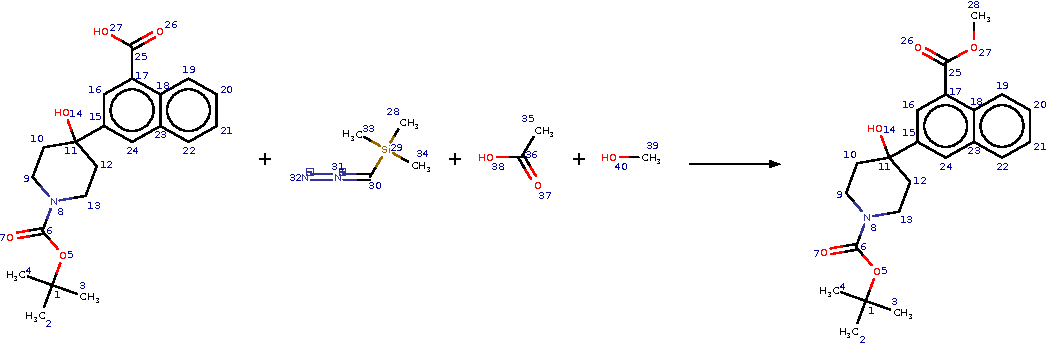
\includegraphics[height=1.2in]{imgs/reaction}
        \caption{Reaction as defined by USPTO SMILES}
    \end{subfigure}
    
    \par\bigskip % force a bit of vertical whitespace 
    \begin{subfigure}[b]{0.8\textwidth}
        \centering
        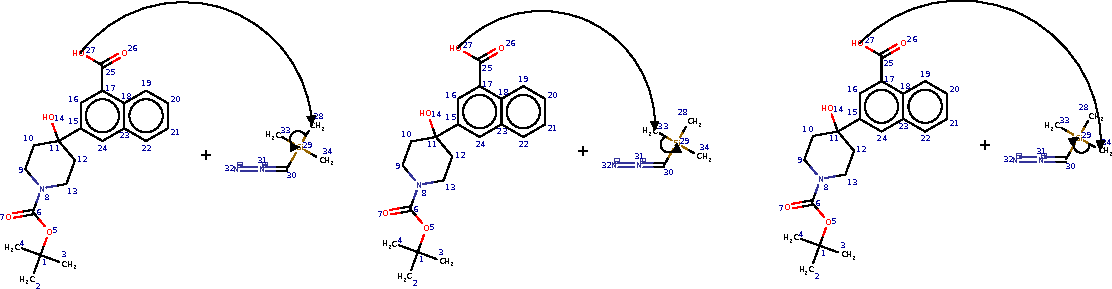
\includegraphics[height=1.2in]{imgs/routes}
        \caption{Possible action sequences that all result in same major product.}
    \end{subfigure}
    \caption{This example shows how symmetry can affect the evaluation of electron paths. In this example, although one electron path is given in the USPTO dataset, after the O (atom map number 27) loses its Hydrogen it can react with any of the CH3 groups in the second reactant to form the same major product. This is why judging purely based on electron path accuracy is misleading.}
    \label{fig:symmetric-reaction-example}
\end{figure*}


\section{Model architecture details}

% these are functions parametrized by NNs: change commands here to match match notation in main paper.
\newcommand{\Ac}{{\mathcal{A}}}
\newcommand{\Hb}{{\mathbf{H}}}

\newcommand{\fEmbed}{f_{\Ac}}
\newcommand{\fAdd}{f_{\textrm{add}}}
\newcommand{\fRemove}{f_{\textrm{remove}}}
\newcommand{\fInitial}{f_{\textrm{initial}}}
\newcommand{\fStop}{f_{\textrm{stop}}}
\newcommand{\fReagEmbed}{f_{\textrm{reagent}}}
\newcommand{\fModules}{\fEmbed, \fAdd, \fRemove, \fInitial,\fStop, \fReagEmbed}

In this section we provide further details of our model architecture and training regime not present in the main paper. 
As mentioned in Section \highlight{REF HERE} of the main paper we have 6 functions, parametrized by NNs, for being able to generate sequences representing electron paths: $\fModules$. 

The function $\fEmbed$ computes node embeddings, $\Hb_{\Ac}$. For this we use Gated Graph Neural Networks (GGNN) \citep{li2016gated, gilmer2017neural}.
 We use 4 propagation steps. 
 The atom features we feed in are detailed in Table \ref{table:atom-features}. These are calculated using RDKit. In total there are 101 features and we maintain this dimensionality in the hidden layers during the propagation steps of the GGNN. Three edge labels are defined: single bonds, double bonds and triple bonds. RDKit is used to Kekulize the reactant molecules. 

\begin{table}
  \caption{Atom features}
  \label{table:atom-features}
  \centering
  \begin{tabular}{ll}
    \toprule
    Feature     & Description      \\
    \midrule
    Atom type & 72 possible elements in total, one hot  \\
    Degree     & One hot (0,   1,   2,   3,   4,   5,   6,   7,  10)  \\
    Explicit Valence     & One hot   (0,   1,   2,   3,   4,   5,   6,   7,   8,  10,  12,  14)    \\
    Hybridization & One hot (SP, SP2, SP3, Other) \\
    H count & integer \\
    Electronegativity & float \\
    Atomic number & integer \\
    Part of an aromatic ring & boolean\\
    \bottomrule
  \end{tabular}
\end{table}


The node features $\Hb_{\Ac}$ are used as inputs by the remaining functions. 
The networks representing $\fAdd$ and $\fRemove$, that operate on each node to produce a action logit, both consist of one hidden layer of 100 units. 
Concatenated onto the node features going into these networks are the current node features belonging to the previous atom in the path.

The network $\fStop$ as described in the main text consists of three functions. 
First similar to \citet[\S B.1]{li2018learning} we  form graph embeddings by a gated sum of projected up node features using the functions $i$ and $j$ which are represented by single linear layers, with $i$ projecting down to one dimension and $j$ to double the dimension of the input node features. 
The function $k$ operates on this embedding to form a logit which goes through a sigmoid function to represent our stop probability. Again we use a single linear layer for this function.

The module $\fReagEmbed$ is similar to $\fStop$, except that the function $k$, again represented by a single linear layer, projects up to a dimensionality of 100.

The final function $\fInitial$ is represented by an MLP with hidden layers of 100 units. When conditioning on reagents the reagent embeddings calculated by $\fReagEmbed$ are concatenated onto the node embeddings and we use two hidden layers. When ignoring reagents we use one hidden layer.

We train everything using ADAM \citep{kingma2014adam} and an initial learning rate of 0.0001, which we decay after 5 and 9 epochs by a factor of 0.1. We use reaction batch sizes of 1.











\bibliography{bibliography}
\bibliographystyle{plainnat}
\end{document}

